\section{\textsc{Разностные методы}}

Относительное позиционирование, также известное как дифференциальное позиционирование, представляет собой совокупность методов, в который измерения от двух или более приёмников и/или спутников вычитаются. 
Подобно комбинированию многочастотных измерений, разностные методы полезны для устранения и минимизации определённых источников ошибок, в том числе ионосферных.
Существует три различных типа дифференциального позиционирования: с использованием одинарных, двойных и тройных разностей. 
Одинарные разности выполняются в одну эпоху измерений для двух спутников и одного приёмника, либо для одного спутника и двух приёмников.
В случе, когда используется два приёмника, расстояние между ними называется \textit{базовой линией (baseline)}.
Для коротких базовых линий (до нескольких километров) ионосферные, тропосферные и эфемеридные ошибки пренебрежимо малы и могут игнорироваться \cite{Seeber2003}. 
Эти ошибки будут расти вместе с увеличением базовой линии, поэтому относительное позиционирование наиболее эффективно для станций, находящихся в непосредственной близости друг от друга.
Двойные разности могут быть сформированы путём вычитания двух отдельных одинарных разностей, т.е. для них необходимо два спутника и два приёмника. 
Тройная разность -- это двойная разность, которая вычитается из той же двойной разности, но в другую эпоху измерений.
Таким образом, для формирования тройной разности все ещё необходимо два спутника и два приёмника, но измерения должны выполняться в последовательные эпохи.
Обозначим через индекс $s=j,k,...$ номера спутников, а через индекс $r=A,B,...$ номера приёмников. 
В таком случае, схема относительного позиционирования соответствует рис. \ref{fig-relative-pos}.
\begin{figure}[h]
\centering    
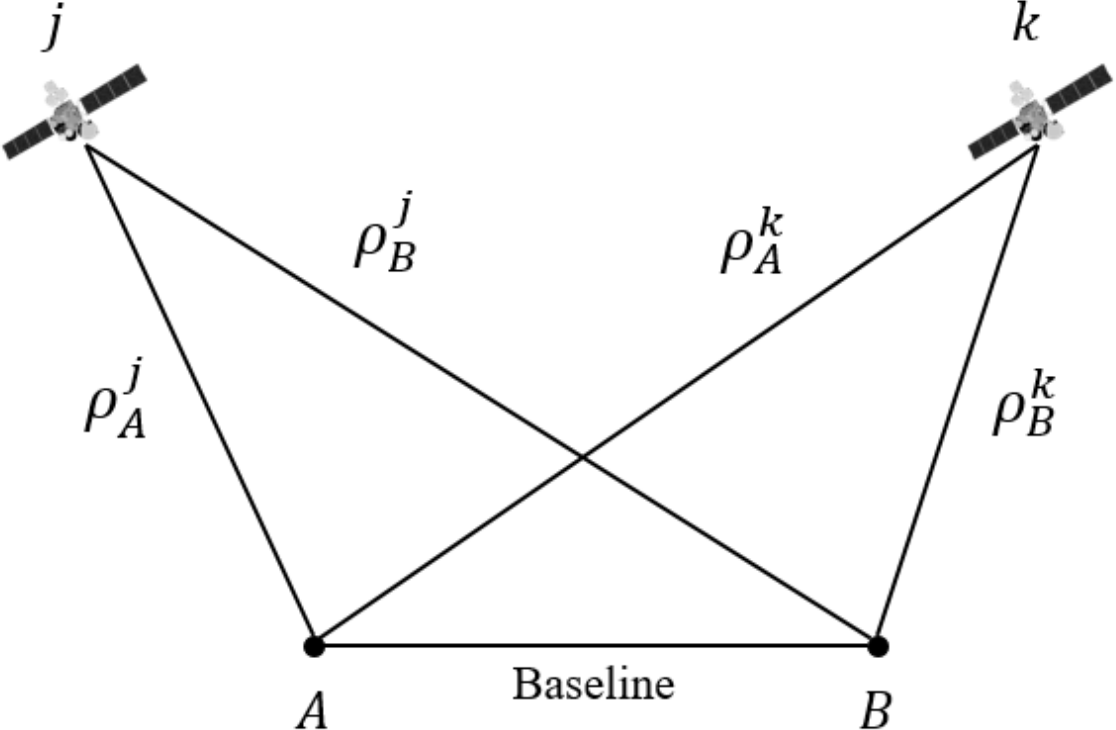
\includegraphics[width=0.5\textwidth]{fig/relative-pos.png}    
\caption{Относительное позиционирования с использованием двух спутников и двух приёмников \cite{Seeber2003}.}
\label{fig-relative-pos}      
\end{figure}  

\subsection*{\textbf{Одинарные разности}}

Относительное позиционирование можно выполнять, используя как измерения псевдодальности, так и фазы несущей.
Рассмотрим принцип формирования одинарных разностей на примере измерений фазы несущей.
Для последующих выкладок введём инструментальные погрешности приёмника $d_{p,r}$ и спутника $d_p^s$, чтобы показать, как они будут устраняться при использовании разностных методов.
Все остальные источники ошибок сгруппируем в одно слагаемое $e_r^s$.
Существуют два разных типа одинарный разностей: между приёмниками и между спутниками.

Для начала рассмотрим одинарную разность между приёмниками, т.е. разность с использованием одного спутника $j$ и двух приёмников $A$ и $B$.
В таком случае, выражения для измерений фазы несущей \eqref{eq-cr2} выглядят следующим образом: 
\begin{equation}
\begin{aligned}
&\Phi_A^j=\frac{1}{\lambda}\left[\rho_A^j+c(\delta_A-\delta^j)+\lambda N_A^j+d_{p,A}-d_p^j+e_A^j\right] \\
&\Phi_B^j=\frac{1}{\lambda}\left[\rho_B^j+c(\delta_B-\delta^j)+\lambda N_B^j+d_{p,B}-d_p^j+e_B^j\right] 
\end{aligned}    
\end{equation}
Вычтя первое выражение из второго и введя обозначение $X_{AB}=X_B-X_A$, получим:
\begin{equation}
\label{eq-single-diff}
\Phi_{AB}^j=\frac{1}{\lambda}\left[\rho_{AB}^j+c\delta_{AB}+\lambda N_{AB}^j+d_{p,AB}+e_{AB}^j\right]    
\end{equation}
Стоит обратить внимание, что слагаемые, относящиеся к инструментальным ошибкам $d_p^j$ и ошибке часов спутника $\delta^j$, исключены.

Теперь рассмотрим одинарную разность между спутниками, т.е. разность с использованием одного приёмника $A$ и двух спутников $j$ и $k$.
В этом случае, выражения для измерений фазы несущей \eqref{eq-cr2} выглядят следующим образом: 
\begin{equation}
\begin{aligned}
&\Phi_A^j=\frac{1}{\lambda}\left[\rho_A^j+c(\delta_A-\delta^j)+\lambda N_A^j+d_{p,A}-d_p^j+e_A^j\right] \\
&\Phi_A^k=\frac{1}{\lambda}\left[\rho_A^k+c(\delta_A-\delta^k)+\lambda N_A^k+d_{p,A}-d_p^k+e_A^k\right] 
\end{aligned}    
\end{equation}
По аналогии, вычтя первое выражение из второго и введя обозначение $X^{jk}=X^k-X^j$, получим: 
\begin{equation}
\label{eq-single-diff2}
\Phi_A^{jk}=\frac{1}{\lambda}\left[\rho_A^{jk}-c\delta^{jk}+\lambda N_A^{jk}-d_p^{jk}+e_A^{jk}\right]    
\end{equation}
В этом случа были устранены аппаратные ошибки $d_{p,A}$ и ошибки часов $\delta_A$ приёмника.

\subsection*{\textbf{Двойные разности}}

Двойные разности формируются простым вычитанием двух одинарных разностей одного типа.
Сформируем одинарную разность наподобие \eqref{eq-single-diff}, но только для спутника $k$, а затем вычтем из нее \eqref{eq-single-diff}.
Введя обозначение $X_{AB}^{jk}=X_{AB}^k-X_{AB}^j$, получим:
\begin{equation}
\label{eq-double-diff}
\Phi_{AB}^{jk}=\frac{1}{\lambda}\left[\rho_{AB}^{jk}+\lambda N_{AB}^{jk}+e_{AB}^{jk}\right]    
\end{equation}
Стоит обратить внимание, что оставшиеся ошибки, связанные с приёмником, полностью исчезли.
Если проделать подобную операцию, но уже с выражением \eqref{eq-single-diff2}, то полностью исчезнуть все ошибки, связанные со спутником.

\subsection*{\textbf{Тройные разности}}

Тройные разности могут быть сформированы печём вычитания двойных разностей в различные эпохи измерений.
Например, рассмотрим двойные разности \eqref{eq-double-diff}, сформированные в две эпохи $t_1$ и $t_2$:
\begin{equation}
\begin{aligned}
&\Phi_{AB}^{jk}(t_1)=\frac{1}{\lambda}\left[\rho_{AB}^{jk}(t_1)+\lambda N_{AB}^{jk}+e_{AB}^{jk}(t_1)\right] \\
&\Phi_{AB}^{jk}(t_2)=\frac{1}{\lambda}\left[\rho_{AB}^{jk}(t_2)+\lambda N_{AB}^{jk}+e_{AB}^{jk}(t_2)\right] 
\end{aligned}
\end{equation}
Вычтя первое выражение из второго и введя обозначение $X_{AB}^{jk}(t_{12})=X_{AB}^{jk}(t_2)-X_{AB}^{jk}(t_1)$, получим:
\begin{equation}
\Phi_{AB}^{jk}(t_{12})=\frac{1}{\lambda}\left[\rho_{AB}^{jk}(t_{12})+e_{AB}^{jk}(t_{12})\right]    
\end{equation}
Как видно, тройные разности полностью устраняют фазовую неопределённость.